\section{Background Research}
\label{sec:background}

%Urged by the concern of users, and building on the gap between battery 
%technology and the power demand of mobile devices, the Green Computing 
%community has tried to answer the need for energy-efficient software 
%Specifically, research has focused on providing tools to developers in 
%order to find and fix the so-called energy bugs, i.e\ the energy greedy 
%portions of code. Alongside high level guidance, novel tools were 
%developed to provide feedback to developers about the energy footprint 
%of their code. These tools can be classified into three types: 
%hardware-based, model-based and software based.

\subsection{High level guidance}

Software optimisation has tended to focus on time, but it was shown in 
\cite{bunse2009choosing} that choosing an energy-efficient 
implementation over a time-efficient implementation allowed more 
operations on a mobile device to be performed. 
\cite{li2014investigation} reviewed a set of coding practices and proved 
that reducing memory usage has a low impact on reducing the energy usage 
of code. Related conclusions were obtained in \cite{sahin2016does} as 
they proved code obfuscation negatively impacts the energy efficiency of 
the underlying software. In \cite{pathak2012energy}, they profiled and 
analysed the energy footprint of six of the top-ten applications on the 
\textit{Google Play Store}. They found that most energy is spent in I/O 
and that most of this energy is due to tail-behaviour. Moreover, it 
appears that I/O energy is spent in a few bundles and that very few 
routines perform I/O. The authors in \cite{linares2014mining} surveyed 
55 applications in order to mine energy greedy calls to the Android API. 
They obtained the cost of 800 API calls and found that the Android API 
was the most energy inefficient part of applications. These findings are 
however, limited by the fact that part of the energy-greedy I/O 
activities are handled in the Java API and therefore don't appear in 
this study. Finally, tail-behaviour was not taken into account.

High level guidance provides a first mean to produce more 
energy-efficient software. However, these findings don't allow 
developers to know which specific parts of code consume the most energy. 
Researchers therefore focussed on developing energy profilers able to 
provide detailed feedback about the energy footprint of applications.

\subsection{Hardware-based profilers}

Hardware-based energy-profilers such as \textit{PowerScope} 
\cite{flinn1999powerscope} and \textit{GreenMiner} 
\cite{hindle2014greenminer} involve the use of power measurement 
platforms, i.e. mobile devices with embedded power sensors monitoring 
the energy drain caused by the running processes. \vlens{}, an 
energy-profiler combining program analysis and statistical modelling to 
provide energy usage information at the source line level was introduced 
in \cite{li2013calculating}. These approaches however, are tied to 
expensive power measurement platforms, involving an overhead for their 
users.

\subsection{Model-based profilers}

Model-based solutions build power models of mobile devices, which are 
further reused away from measurement platforms to profile the energy 
footprint of applications. \textit{eCalc} \cite{hao2012estimating} 
assumes the availability of a CPU power profile containing the energy 
drain associated with each CPU instruction in order to provide drain 
caused by the CPU at the method granularity. \textit{PowerBooter} uses 
battery voltage sensors and the knowledge of the battery behaviour to 
automate the power model generation and \textit{PowerTutor} further uses 
this model to compute the energy costs \cite{zhang2010accurate}. 
\textit{TailEnder} provides models focussing on the drain of I/O 
components, namely 3G and GSM. \eprof{} \cite{pathak2012energy} focusses 
on mapping the drain caused by hardware components with accounting 
entities such as processes, threads and routines. For each entity, 
\eprof{} produces an energy tuple \texttt{(utilisation\_draw, 
tail\_mode\_draw)} and is therefore one of the few contributions 
accounting for tail energy and comparing it to utilisation drain. They 
also present methods to generate these power models by correlating 
certain behaviours with specific power states and identifying these 
behaviours as trigger conditions on the finite state machine 
\cite{pathak2011fine}. Model-based techniques suffer one major drawback: 
the underlying power models are specific to the profiler and are 
therefore not widespread nor publicly available.

\subsection{Software-based profilers}

Software-based solutions were introduced to allow for portable and 
widely accessible energy-profilers. They do not require any knowledge of 
the device behaviour or to have access to specific hardware. Users 
usually provide their application alongside a test scenario. Based on 
the findings in \cite{linares2014mining}, \cite{jabbarvand2015ecodroid} 
introduced \textit{EcoDroid}, an energy profiler that focuses on ranking 
the applications instead of providing energy estimates. The Power 
Estimation Tool for Android Application (\petra{}) uses new tools of the 
Android Open Source project focussing specifically on energy profiling 
\cite{petra}. \petra{} simulates a typical execution of the tested 
application on an actual device using a user-provided script. The 
execution trace is recorded using \texttt{dmtracedump} and the 
\batterystats{} history is collected using \dumpsys{}. \petra{} finally 
replays these files to compute the battery drain during the execution of 
each method and provides the user with the energy estimates at the 
method level.

\Orka{} \footnote{\Orka{} is now available at 
\url{https://github.com/acornet/orka}} is one of the first 
software-based energy profilers \cite{westfield2016orka}. It takes an 
Android application and a dynamically created execution trace to provide 
the energy usage estimations as feedback. The energy cost of a routine 
is calculated using the energy costs of the Android API calls (from 
\cite{linares2014mining}). Following the background research, extending 
Orka appeared as the most viable solution in order to fulfil the 
aspirations of this work. The basic workflow of \Orka{}, presented in 
Figure \ref{fig:orkaworkflow}, is divided into three main steps: (i) the 
application is instrumented in order to log the API calls, (ii) the 
instrumented application is then run on the Android emulator using a 
user-supplied \monkeyrunner{} script, and (iii) the execution traces are 
analysed and the results are presented to the user. The execution 
analysis is done by using the logs and the \batterystats{} data and is 
used to calculate the total cost of a routine which is obtaining by the 
following relation: $cost(routine) = \sum_{API \in routine} cost(API)$. 
The \batterystats{} file also gives the breakdown by component of the 
hardware energy usage.

\begin{figure}
\centering
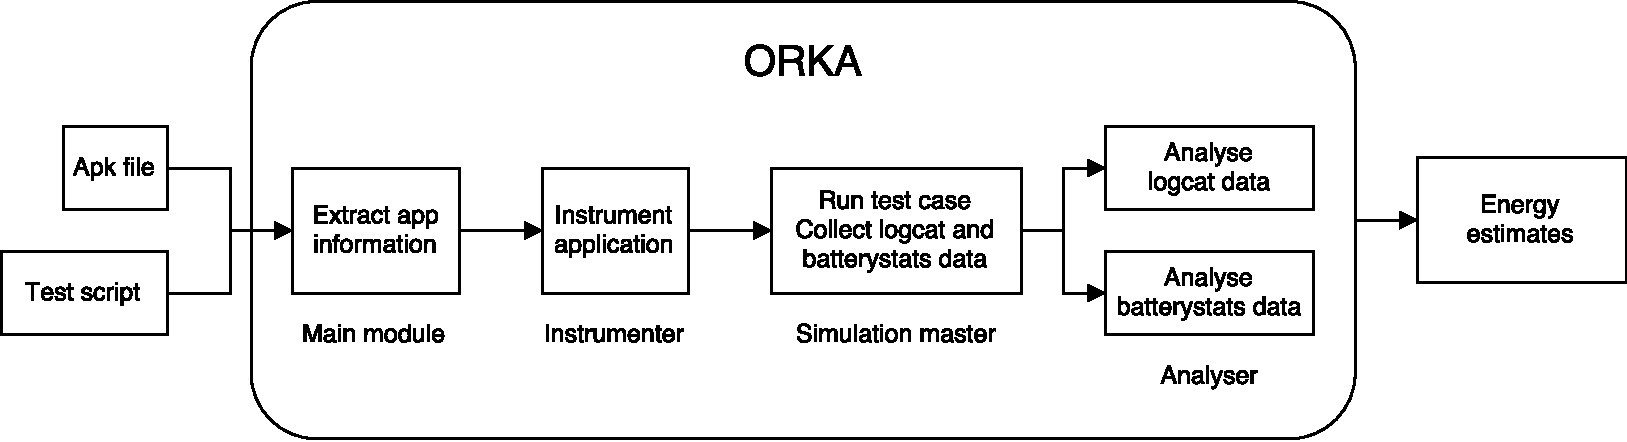
\includegraphics[width=0.5\textwidth]{figures/orkaworkflow.pdf}
\caption{Basic workflow of \Orka{}}
\label{fig:orkaworkflow}
\vspace {-0.32in}
\end{figure}
